\section{Experiments}

\subsection{Data and Protocol}

We evaluate only the TSRS\_RSNA-Epiphysis subset. The indexed labels are converted in isolated output directories; the original images and annotations remain unchanged. The fixed split contains 875 training and 96 original-validation radiographs. A separate clean-test-v2 split is reserved for final evaluation and is not used for threshold selection, checkpoint selection, or the results reported here.

Both systems use a two-dimensional PlainConvUNet configured by nnU-Net, a $512\times512$ patch, batch size 2, and the same 875/96 split. A 30-epoch matched run is followed by a 150-epoch mature run initialized from the corresponding best weights with a reset optimizer and learning-rate schedule. We select checkpoints using nnU-Net's exponentially smoothed foreground Dice criterion. The control predicts background and bone; the seam model predicts background, bone, and seam.

\subsection{Metrics}

The frozen R201 protocol reports Dice, IoU, precision, recall, Boundary IoU, Boundary F1, Surface Dice at 2 and 5 pixels, HD95, and average symmetric surface distance. Pixel distances are reported because reliable physical spacing is unavailable. We additionally report two task-specific diagnostics. Gap-region false-positive rate measures foreground predictions in a nine-pixel dilated background band around the ground truth. Component merge rate is operationally defined as the fraction of images for which the predicted binary mask contains fewer connected components than the binary ground truth:
\begin{equation}
\mathrm{CMR}=\frac{1}{N}\sum_{i=1}^{N}\mathbb{1}[C(\hat{\B}_i)<C(\B_i)].
\end{equation}
It is an image-level component under-count diagnostic, not a universal instance-segmentation metric. Component-count MAE reports $|C(\hat{\B})-C(\B)|$.

\subsection{Quantitative Results}

\begin{table*}[t]
\centering
\small
\caption{Mature matched comparison on 96 original-validation images. Higher is better for Dice, recall, Boundary IoU/F1, and Surface Dice; lower is better for gap FP, CMR, count MAE, HD95, and ASSD.}
\label{tab:main}
\begin{tabular}{lccccccccccc}
\toprule
Method & Dice & Recall & BIoU & BF1 & SD2 & SD5 & Gap FP & CMR & Count MAE & HD95 & ASSD\\
\midrule
Binary nnU-Net & \textbf{.8980} & \textbf{.8991} & .2343 & .3731 & .6501 & .9004 & .1873 & .5104 & \textbf{2.333} & \textbf{16.35} & \textbf{6.17}\\
Seam supervision & .8974 & .8966 & \textbf{.2350} & \textbf{.3742} & \textbf{.6515} & \textbf{.9008} & \textbf{.1832} & \textbf{.4271} & 2.438 & 33.39 & 6.98\\
\bottomrule
\end{tabular}
\end{table*}

Table~\ref{tab:main} shows a targeted change rather than uniform improvement. CMR falls by 8.33 percentage points, from 51.04\% to 42.71\%, and gap-region FP falls by 0.0041. Boundary IoU, Boundary F1, and Surface Dice improve slightly. Dice changes by $-0.0006$, indicating that the component improvement is not explained by a large loss of overlap. However, recall decreases by 0.0025, count MAE increases by 0.104, and HD95 nearly doubles. The seam target therefore suppresses some false bridges but also creates or exposes isolated boundary errors.

\subsection{Qualitative Analysis}

\begin{figure*}[t]
\centering
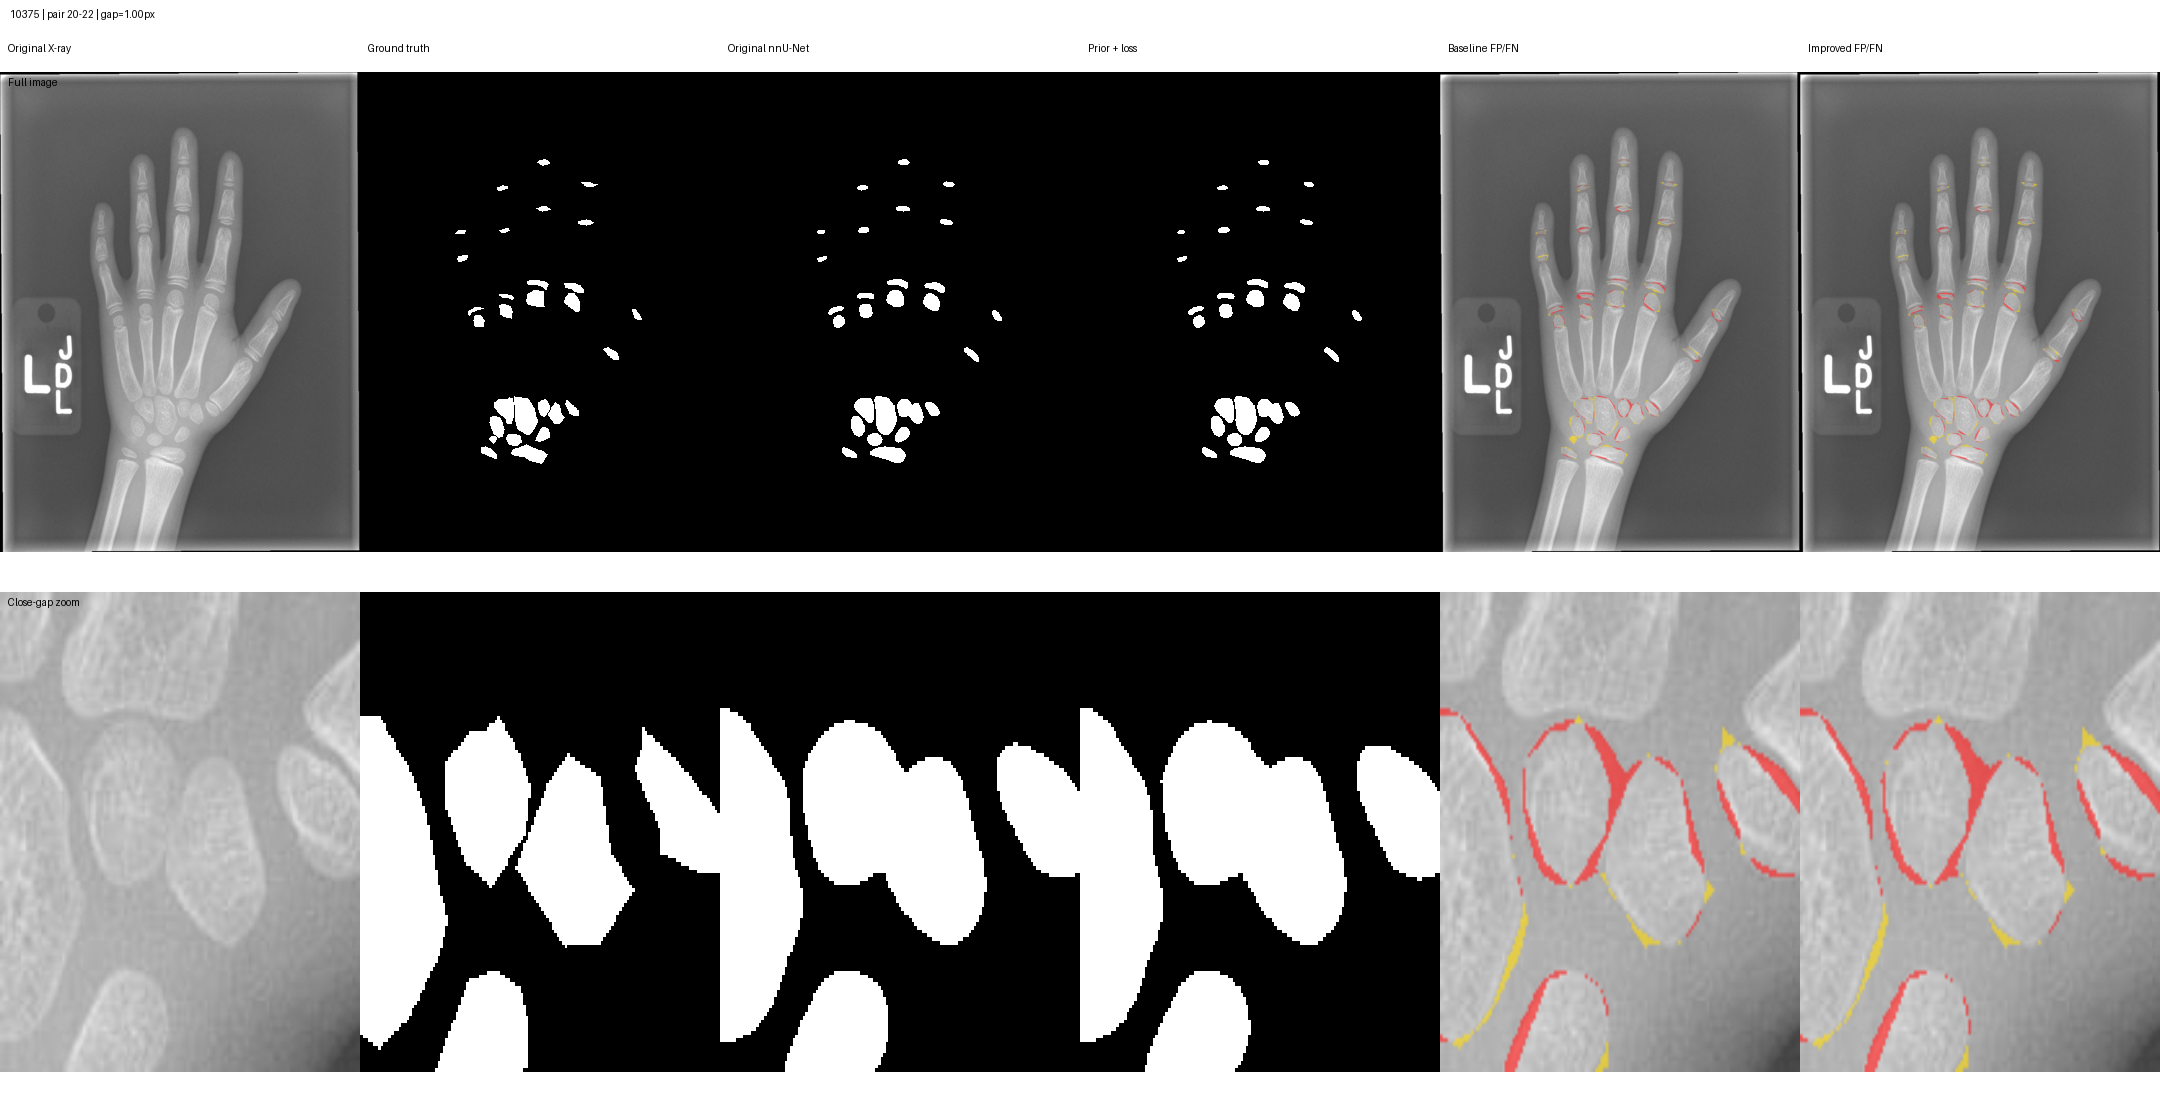
\includegraphics[width=\textwidth]{figures/qualitative_10375.png}
\caption{Matched qualitative comparison. The top row shows the full radiograph, label, mature binary nnU-Net, seam-supervised nnU-Net, and error overlays. The bottom row magnifies a one-pixel-gap hard case. Red denotes false-positive foreground and yellow denotes false-negative foreground. The seam model changes the narrow separation geometry, but residual boundary displacement remains.}
\label{fig:qualitative}
\end{figure*}

Figure~\ref{fig:qualitative} illustrates why overlap and component diagnostics must be reported together. Predictions with similar union area may differ at a narrow bridge. Conversely, a method can remove a bridge by eroding foreground, which motivates the simultaneous recall, surface-distance, and component-count checks.
